\chapter{Introduction}

\begin{wrapfigure}{R}{0.2\textwidth}
	\caption{KuKa LWR Arm with Shadow C5 Hand installation\label{fig:armwithhand}}
	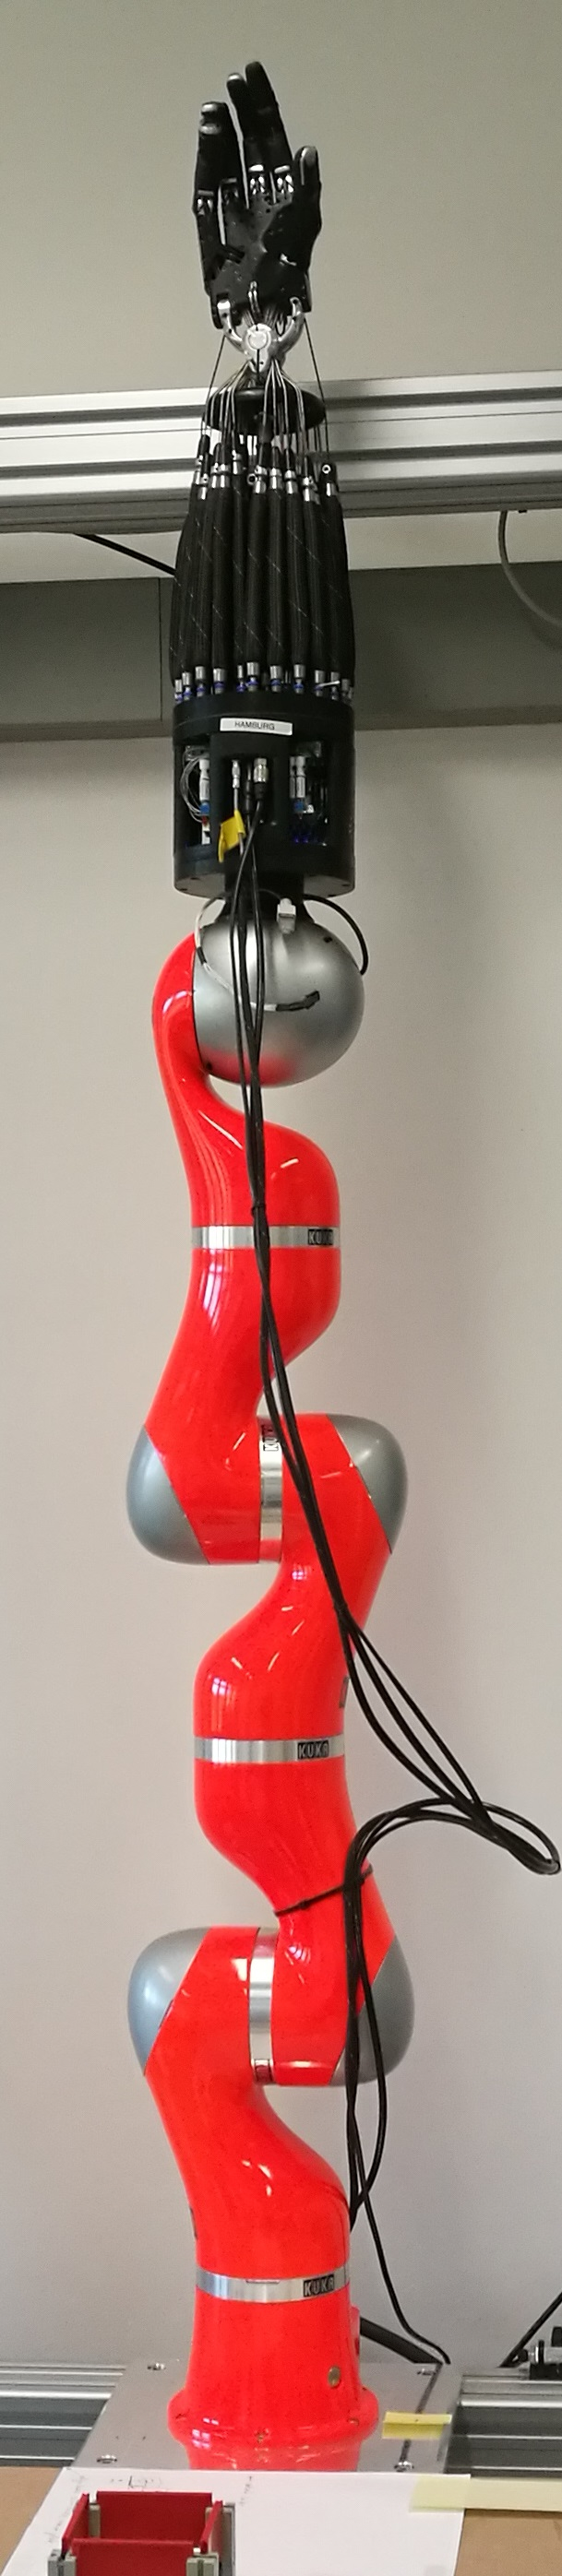
\includegraphics[width=0.2\textwidth]{assets/chpt_intro/lwr_c5hand.jpg}
\end{wrapfigure}

\section{Motivation}

Controlling dexterous robot hands is a big challenge of robotics, but their usage has a variety of obvious advantages: The similarity to a human hand enables it to grasp objects in nearly all positions and poses the real human hand could. Especially for complex manipulation tasks, where a simple robotic grasper with just a pair of pliers is not sufficient, the larger amount of degrees-of-freedom comes into action. Also, users might be able to better plan actions when they are controlling a device similar to their own hands, meaning the main task for them is to use a control interface to execute actions they would otherwise execute with their own hands. Additionally, the robotic hand potentially has more advantages than the human hand, higher degrees-of-freedom, more strength or special fingertips adding more friction and by that enabling grasping of more (e.g. very sleek) different materials. This would give users the ability to perform tasks as they would with their own hands but with less effort or more effective.

\section{Objectives of this thesis}

Within this thesis, a touch-interface for controlling such robotic hands shall be developed, taking advantage of the multi-touch capabilities of modern mobile tablet computers. The user shall be able to control the position of the robotic hand (using the connected robotic arm) and grasp objects with it. All actions shall be mapped to corresponding multi-touch gestures the user can easily understand and learn.

The hardware used within this bachelor thesis is a \textit{Shadow Dexterous Hand C5/C6} by the Shadow Robot Company. It has five fingers controlled by electrical or pneumatic muscles using 20 degrees-of-freedom\cite{web:robothand:spec}. The hand is connected to a robotic arm (\textit{KUKA Lightweight Robot}) allowing it to also be moved in space (See Figure \ref{fig:armwithhand} for an image of the installation).

As a control device an off-the-shelf android tablet will be used, as these devices have become very widespread and - thanks to this - relatively affordable. With screen sizes of 10 inches and above combined with the capability to record more than 5 independent touch pointers and a number of additional sensors (gyroscope, orientation, ...) and feedback actuators (vibration, sound, ...) they make a good choice for a versatile control device.

Specifically, development during this thesis will take place on a \textit{Samsung Galaxy Tab S3}. It has a screen size of 9.7 inches\cite{samsung:galaxytabs3} with a resolution of 2048x1536 pixels accompanied by a 2.15GHz Quad-Core processor. These properties give it the ability to also perform some calculation-heavy tasks locally, giving the overall application a better performance. The used Android tablet runs Android 7.0. One goal of this thesis is to make the control application available to a broad variety of devices. Because of this, the application shall run on Android down to Version 4.3 and up to the current 7.0.

A native Android application will be developed and run directly on the tablet. As a programming language Java is chosen, as it is the language natively used on Android. Multiple approaches to the problem will be implemented to give users and researchers the ability to test and evaluate multiple methods against their usability, effectiveness and user-friendliness.

\section[Outline]{Outline}

In Chapter \ref{chap:basics} a brief overview over the technology used during the development of this thesis will be described and explained to give the reader a profound basis of knowledge to understand the processes and decisions described later. Chapter \ref{chap:concepts} depicts the concepts and architectural design process decisions made for later development. The implementation is then described in detail within Chapter \ref{chap:implementation}. Proposals for user studies and usability evaluations are then made in Chapter \ref{chap:eval}, as they are not part of this thesis.

\chapter{Related work}

A lot of research is and was done in the field of remote-controlling robots with generic devices. This is most probably the case due to them being ubiquitous and well-known by common users. This is important as more and more robots have entered the personal living spaces of users during the last 2 decades\cite{Forlizzi2006} which have to be controlled by untrained persons with the least possible amount of learning. This leads to the need of very easily understandable user interfaces and a small amount of complexity in the possible controls. 

One approach to reduce complexity in controlling a robot with a high amount of degrees-of-freedom (DOF) is described in \cite{Bernardino2013}. The researchers conducted a principal component analysis (PCA) on different grasping hand poses. The calculated components can then be used to control a device with e.g. 22 DOF by just 2-3 parameters. As this thesis is partly based on this approach and the given research, more explanation can be found in Chapter \ref{chap:concepts}. Apart from this analytical approach another part of this thesis is based on \cite{conf:humanoids:TohHLBZP12} where researchers developed a method to directly map finger positions on a tablet computer to those on a robotic hand. These are the two main approaches examined in this thesis.

Other ideas to teleoperate robots with generic devices are numerous. A similar approach is to control a mobile robot using an android device by tilting it\cite{Akupati2017}. The idea here is to simulate a steering wheel of a car to move a car-like robot. 

As the fields of virtual reality (VR) and augmented reality (AR) gain more and more attention, different approaches to remotely control robots assisted by such VR systems come up. Hashimoto et al. developed a software called TouchMe, displaying a video image of a robot, allowing to directly alter a robot model perfectly laid over the video image using simple drag and drop actions on a touchscreen\cite{Hashimoto2013}. Krupke et al. took the approach one step further by displaying the virtual environment on a head mounted device (HMD, also referred as \textit{VR glasses}). The HMD displays a virtual representation of the manipulated device, allowing the controller to look at the scene from arbitrary angles. Fine control was implemented by putting the controller's hand into a virtual sphere and recording hand movement while mapping it to movements of the controlled robot.
